\input format.tex

\usepackage{graphicx}
\graphicspath{{cores/}}

\usepackage{environ}
\usepackage{colortbl,array,booktabs}
\usepackage{tabularx}

\colorlet{TablaBordeSuperior}{topcolor}
\colorlet{TablaBordeInferior}{topcolor}
\colorlet{TablaCentroSuperior}{blue!1}
\colorlet{TablaCentroInferior}{blue!20}
\colorlet{FuenteCabeceraTabla}{white}

\newcolumntype{M}[1]{>{\centering\arraybackslash}m{#1}}
%\newcommand{\tabularxcolumn}[1]{>\arraybackslash}m{#1}}

\tcbset{rtab/.style={
freelance,
frame code={
 \path[top color=topcolor,bottom color=topcolor]
   ([yshift=-#1*(\baselineskip+2pt)]interior.north west) --
   ([yshift=-#1*(\baselineskip+2pt)]interior.north east) {[sharp corners]--
    ([yshift=3pt]interior.north east) --
    ([yshift=3pt]interior.north west)} -- cycle;

  },
interior code={},
 }
}

\newcommand\fuentecabecera[1]{\textcolor{black}{\textbf{#1}}}

\begin{document}

\vspace*{8mm}
%% 各章节
\setlength{\arrayrulewidth}{.2pt}
\fontsize{8.8pt}{11pt}\selectfont
\color{gray2}

\noindent{\bf{潜在疾病风险}}

\begin{spacing}{1.5}
\begin{LRaside}[.8]{\fontsize{8.8pt}{11pt}\selectfont 检测说明}
\noindent
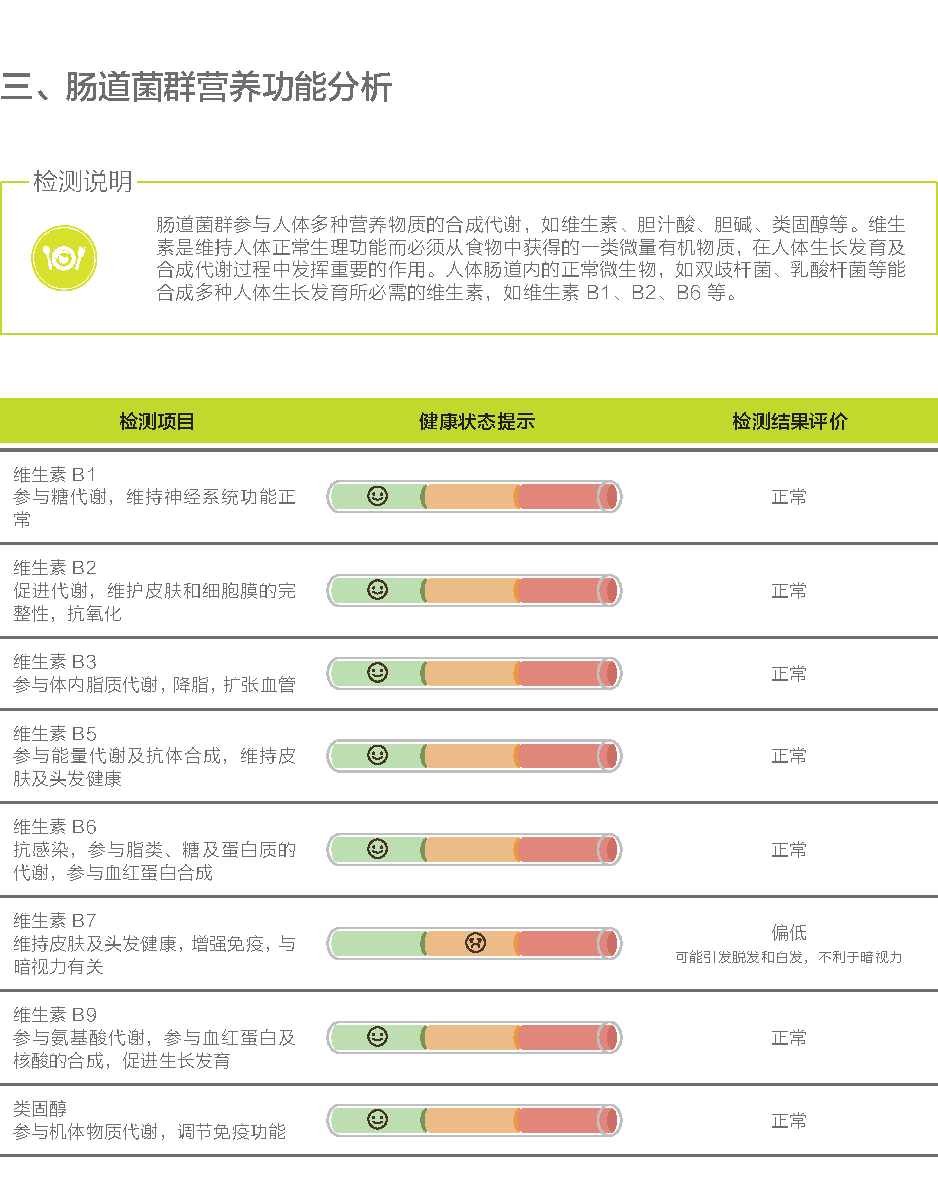
\includegraphics[width=\linewidth]{yingyanggongneng.pdf}
\asidebreak %
{\fontsize{8pt}{11pt}\selectfont 肥胖不仅给个人形象带来负面影响,更重要的是会带来潜在的疾病风险。2015年减肥药物临床实践指南已明确指出,BMI≥30的成年肥胖患者每年应体检筛查Ⅱ型糖尿
病、心血管疾病、高血压、高脂血症、阻塞性睡眠呼吸暂停、非酒精性脂肪肝疾病、骨关节炎和抑郁症疾病。俗话说:“一胖生百病”,这些潜在的疾病风险已成了肥胖患者
最担心的问题。通过肠道菌群检测可以有效预测疾病的潜在风险,真正实现了早检测、早预防、更健康。}
\end{LRaside}
\end{spacing}

\noindent 检测结果

\begin{tctabularx}{tabularx={m{4cm}<{\centering}m{6.6cm}<{\centering}m{4cm}<{\centering}}}
&&
\\[-6pt]
\cellcolor{topcolor} \raisebox{2.614pt}{\color{gray2}\bf 检测项目} &
\cellcolor{topcolor} \raisebox{2.614pt}{\color{gray2}\bf 健康状态提示} &
\cellcolor{topcolor} \raisebox{2.614pt}{\color{gray2}\bf 检测结果评价}
\end{tctabularx}

\vspace*{-4.25mm}
\fontsize{8pt}{11pt}\selectfont
\arrayrulecolor{gray2}
\begin{longtable}{m{4cm}<{\centering}m{6.6cm}<{\centering}m{0cm}@{}m{4cm}<{\centering}}

\hline
%\parbox[c]{\hsize}{\vskip7pt {\lantxh 2型糖尿病\\ \bahao HASH(0x1c705a8)} \vskip7pt} 
\parbox[c]{\hsize}{\vskip7pt {\lantxh 2型糖尿病} \vskip7pt} & \parbox[c]{\hsize}{\vskip7pt\centerline{\raisebox{-1.5ex}{
\includegraphics[width=5cm,height=0.55cm]{diseasebar.pdf}}}\vskip7pt} &
\hspace*{-5.03cm}\raisebox{-0.55ex}{
\includegraphics{smile.pdf}} &
\begin{minipage}{4cm}\begin{center}{{\lantxh 正常} }\end{center} \end{minipage} \\
\hline
%\parbox[c]{\hsize}{\vskip7pt {\lantxh 动脉粥样硬化\\ \bahao HASH(0x1c707e8)} \vskip7pt} 
\parbox[c]{\hsize}{\vskip7pt {\lantxh 动脉粥样硬化} \vskip7pt} & \parbox[c]{\hsize}{\vskip7pt\centerline{\raisebox{-1.5ex}{
\includegraphics[width=5cm,height=0.55cm]{diseasebar.pdf}}}\vskip7pt} &
\hspace*{-5.03cm}\raisebox{-0.55ex}{
\includegraphics{smile.pdf}} &
\begin{minipage}{4cm}\begin{center}{{\lantxh 正常} }\end{center} \end{minipage} \\
\hline
%\parbox[c]{\hsize}{\vskip7pt {\lantxh 高血压\\ \bahao HASH(0x1c709b0)} \vskip7pt} 
\parbox[c]{\hsize}{\vskip7pt {\lantxh 高血压} \vskip7pt} & \parbox[c]{\hsize}{\vskip7pt\centerline{\raisebox{-1.5ex}{
\includegraphics[width=5cm,height=0.55cm]{diseasebar.pdf}}}\vskip7pt} &
\hspace*{-2.83cm}\raisebox{-0.55ex}{
\includegraphics{cry.pdf}} &
\begin{minipage}{4cm}\begin{center}{{\lantxh 高风险} }\end{center} \end{minipage} \\
\hline
%\parbox[c]{\hsize}{\vskip7pt {\lantxh 非酒精性脂肪肝\\ \bahao HASH(0x1c70b48)} \vskip7pt} 
\parbox[c]{\hsize}{\vskip7pt {\lantxh 非酒精性脂肪肝} \vskip7pt} & \parbox[c]{\hsize}{\vskip7pt\centerline{\raisebox{-1.5ex}{
\includegraphics[width=5cm,height=0.55cm]{diseasebar.pdf}}}\vskip7pt} &
\hspace*{-5.03cm}\raisebox{-0.55ex}{
\includegraphics{smile.pdf}} &
\begin{minipage}{4cm}\begin{center}{{\lantxh 正常} }\end{center} \end{minipage} \\
\hline
\end{longtable}

\vspace*{3mm}
\begin{spacing}{1.5}
\begin{LRaside}[.8]{\fontsize{8.8pt}{11pt}\selectfont 结果分析}
\noindent

\includegraphics[width=\linewidth]{result_fenbu.pdf}
\asidebreak %
\fontsize{8pt}{11pt}\selectfont 根据肠道菌群检测结果提示,会增加高血压的风险,请引起关注,需要避免这些疾病的高危因素,注意调理肠道菌群结构,改善肠道环境,降低疾病风险,还需注意定期检查。

\end{LRaside}
\end{spacing}

\noindent\fontsize{7.5pt}{11pt}\selectfont {(注:本检测仅作为健康评估,不作为临床诊断,注意正常并不意味着无疾病发生的可能;高风险也不意味着一定发生此病。)}

\end{document}
